\section{EVALUATION}
\label{sec:eval}

\begin{figure}[!t]
  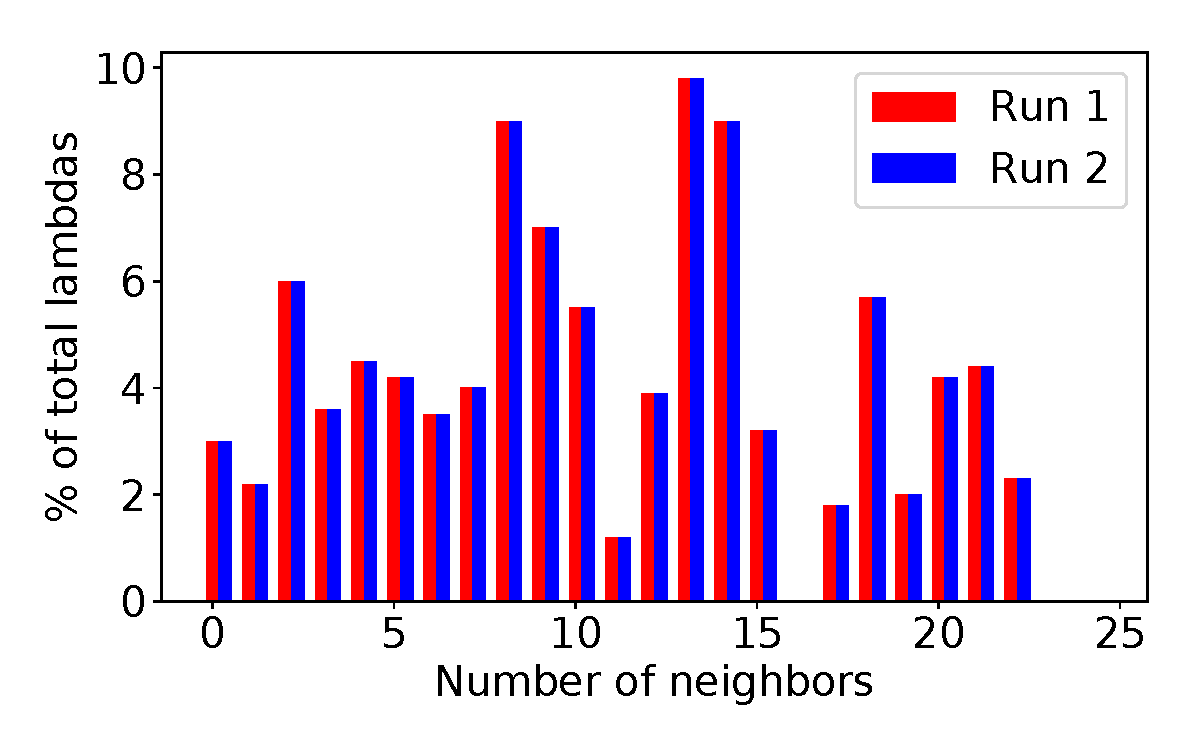
\includegraphics[width=.99\linewidth]{fig/correlation.pdf}
  \caption{This figure shows the fraction of lambdas by the number of neighbors 
  they identify for two independent runs that use same set of underlying AWS
  containers. The perfect correlation shows that both runs depict the co-residence 
  status of those containers regardless of the lambdas that ran on them, providing
  evidence for the correctness of our approach.
  \todo{make it print friendly}
\label{fig:correlation}}
\end{figure}

In this section, we evaluate the effectiveness of both our co-residence detection
technique and our covert channel.

\subsection{Co-residence protocol}
First, we examine our co-residence detector with respect to reliability and
scalability, the desirable detection properties mentioned in
section~\ref{sec:methodology}.  We run all of our experiments with AWS
lambdas~\cite{awscloud}. Though we decide to focus on only one of the cloud
providers as a case study, we have previously shown in
section~\ref{sec:methodology} that this covert channel exists on the other
clouds, and thus these experiments can be replicated on their serverless
functions as well. We use the C++ runtime in AWS lambdas as it allows pointer
arthmetic that is required to access the covert channel.\todo{add note about
this fulfilling fast requirement?}

\subsubsection{Setup}
\label{subsec:expsetup}
For each experiment, we deploy a series of instances from an AWS lambda
account. Once deployed, each instance participates in the first phase of the
protocol as noted in section~\ref{sec:protocol:complexity}, thereby learning the
largest ID of their neighbors. As bit-flip errors are possible, we repeat the
same phase for two more (independent) "rounds" and take the majority result to
record the ID seen by this instance.  If all three rounds result in different
IDs, we classify this instance as erroneous and report it in the error rate. We
group all the instances that saw the same ID as successful and neighbors. We
repeat the experiments for different lambda sizes and in various cloud regions.
\todo{add cost here}

\subsubsection{Reliability}
We consider the results of the technique reliable when 1) most of the deployed
instances successfully see the same result in majority of the independent rounds
(indicating lesser bit-flip errors) and 2) the resulting co-resident groups we
see match the ground truth.  For goal \#1, we ran an experiment with 1000 AWS
lambdas and compared the error rate across different lambda sizes (the error
rate indicates the fraction of these 1000 lambdas that did not have a majority
result). Figure~\ref{fig:errorrates} indicates that smaller lambdas exhibit many
more errors.  This is expected because, as discussed in section
\ref{sec:method:noise}, these lambdas experience lossy communication making it
harder for our technique to sense contention. Lambdas that are 1.5 GB and
larger, though, exhibit a 100\% success rate.
\todo{rebuttal: clarify false postives and negatives}

\textbf{Correctness} 
\todo{promised clarity here in rebuttal}
To determine correctness, we require ground truth on which instances are
co-resident with one another. While such information is not available, we are
able to ascertain correctness of our approach by utilizing an AWS caching
mechanism. On AWS, each lambdas runs in a dedicated container (sandbox).  After
execution, AWS caches these containers in order to reuse
them~\cite{awscontainerreuse} for repeat lambdas and mitigate "cold start"
latencies. For C++ lambdas, we found that the data structures declared in the
global namespace are tied to containers and are not cleared on each lambda
invocation, so we can use a global array to record all the lambdas that were
ever executed in a particular container. This indicates that, for a given
lambda, we can precisely note all the lambdas that previously ran in the same
container (aka predecessors).  Using this, we are able to validate that
identical experiments repeated within minutes of one another will use the same
set of underlying containers for running the deployed lambdas. Since lambda
co-residence is essentially co-residence of their containers, and given that
containers persist across experiments that are executed within minutes of one
another, lambda co-residence results must agree with the co-residence of their
underlying containers for true correctness.


\begin{figure}[!t]
  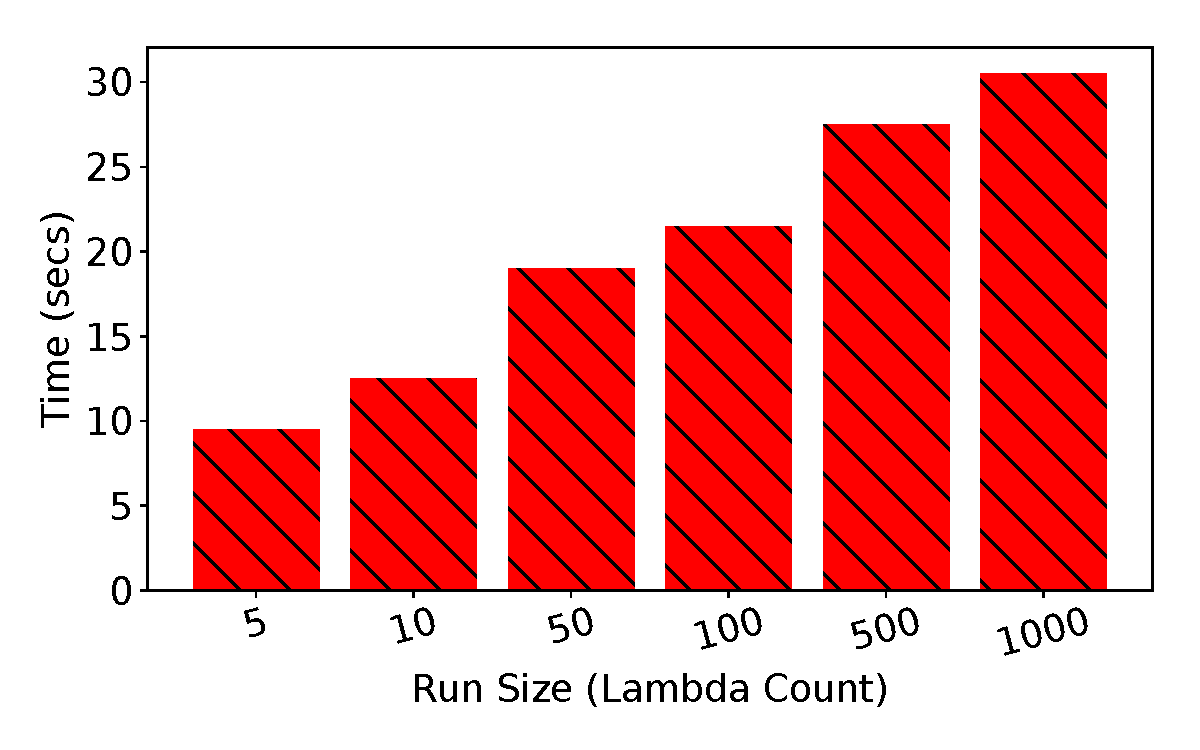
\includegraphics[width=.99\linewidth]{fig/runtimes.pdf}
  \caption{We present the average execution time of the lambdas for co-resident
  runs with a varying number of lambdas. The execution time increases
  logarithmically with the number of lambdas demonstrating the scalability of
  co-residence detection with our technique.
\label{fig:runtimes}}
\end{figure}


% Figures from the next section
% Moved here for formatting

\begin{figure*}[!t]
  \begin{subfigure}{.33\textwidth}
    \centering
    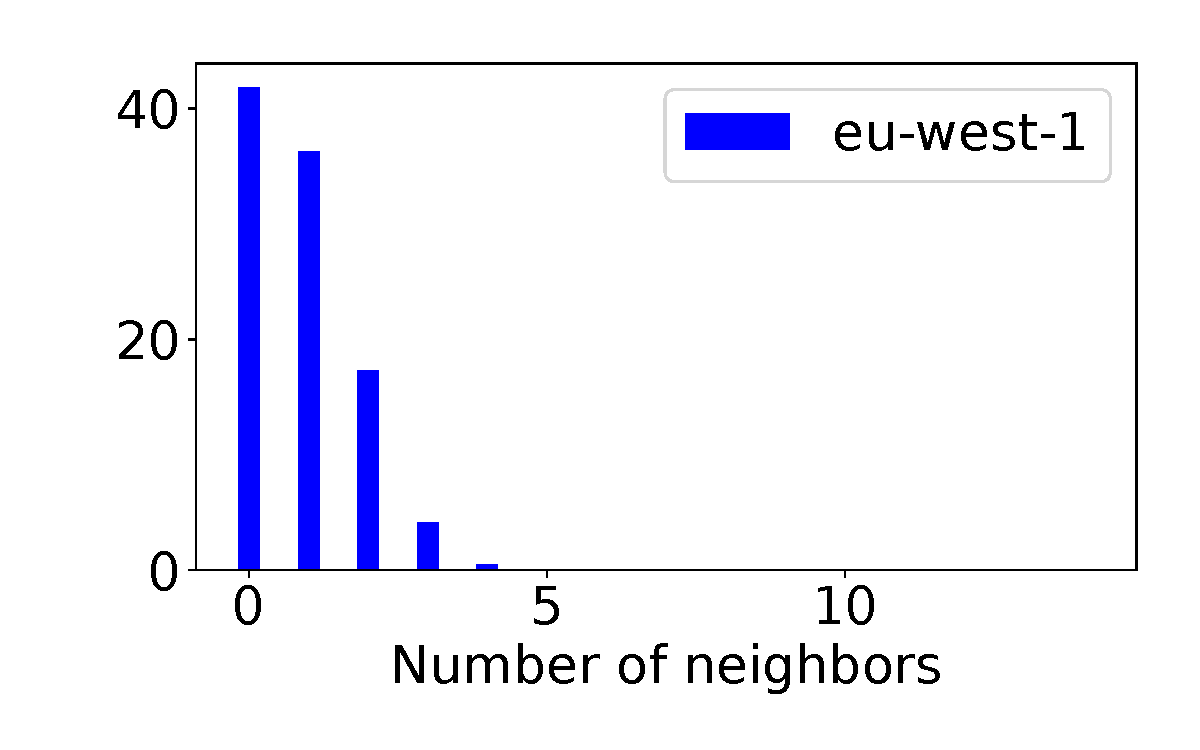
\includegraphics[width=.99\linewidth]{fig/colocation-eu-west-1.pdf}
  %   \caption{1a}
  %   \label{fig:sfig1}
  \end{subfigure}%
  \begin{subfigure}{.33\textwidth}
    \centering
    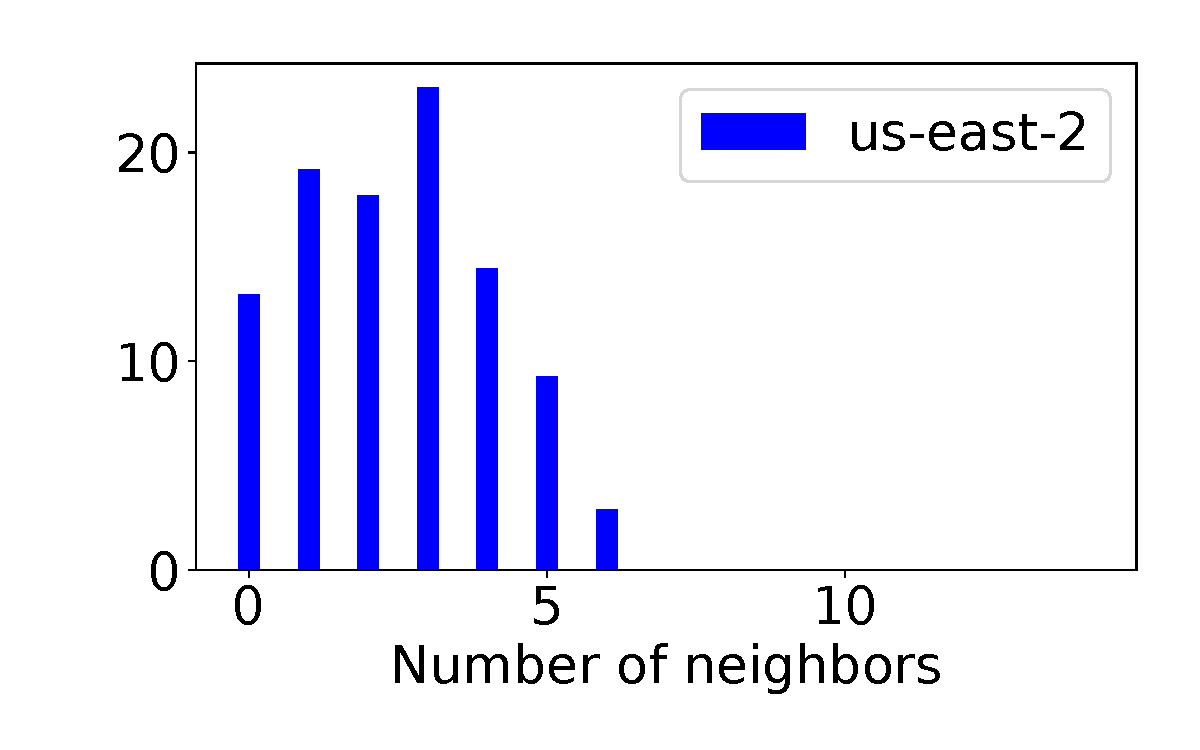
\includegraphics[width=.99\linewidth]{fig/colocation-us-east-2.pdf}
  %   \caption{1b}
  %   \label{fig:sfig2}
  \end{subfigure}
  \begin{subfigure}{.33\textwidth}
    \centering
    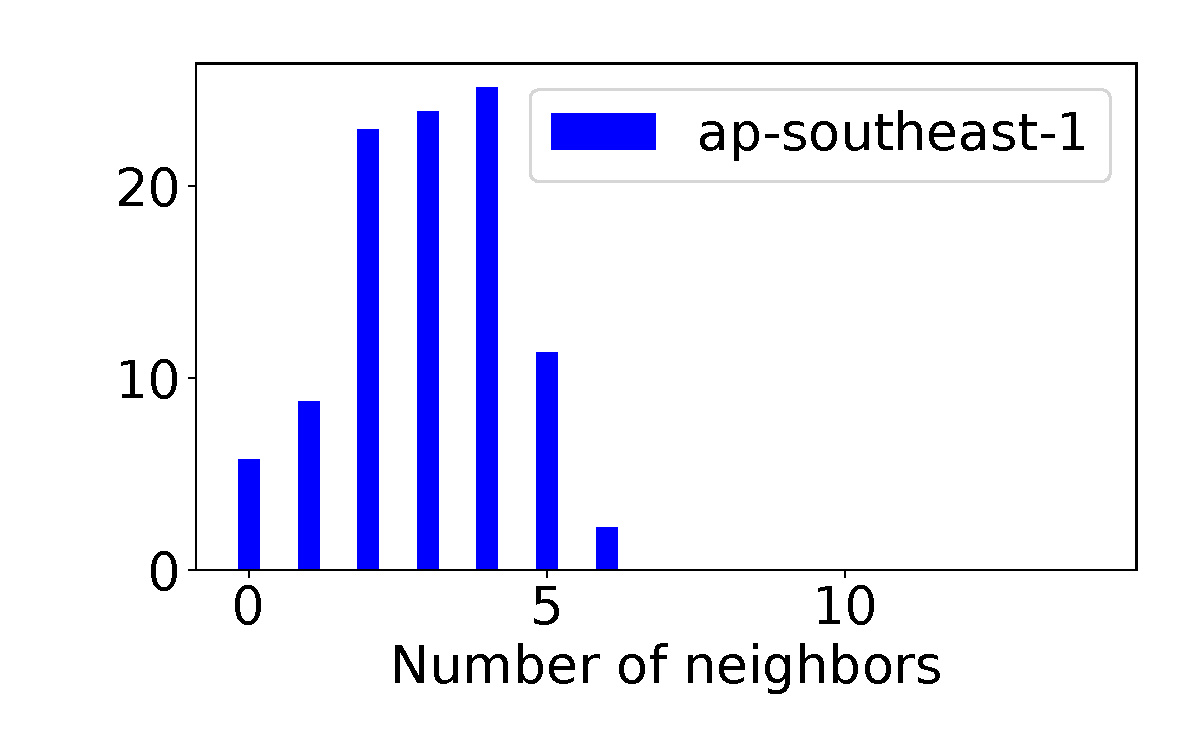
\includegraphics[width=.99\linewidth]{fig/colocation-ap-southeast-1.pdf}
  %   \caption{1b}
  %   \label{fig:sfig2}
  \end{subfigure}
  
  \begin{subfigure}{.33\textwidth}
    \centering
    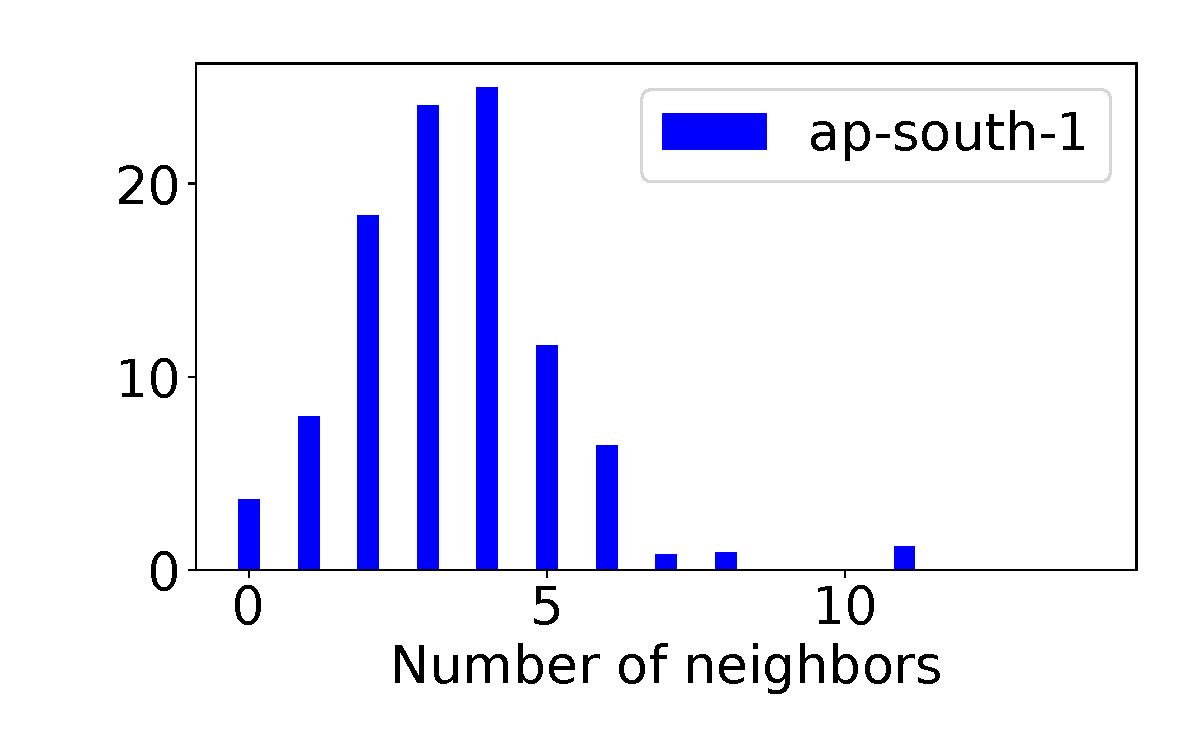
\includegraphics[width=.99\linewidth]{fig/colocation-ap-south-1.pdf}
  %   \caption{1a}
  %   \label{fig:sfig1}
  \end{subfigure}%
  \begin{subfigure}{.33\textwidth}
    \centering
    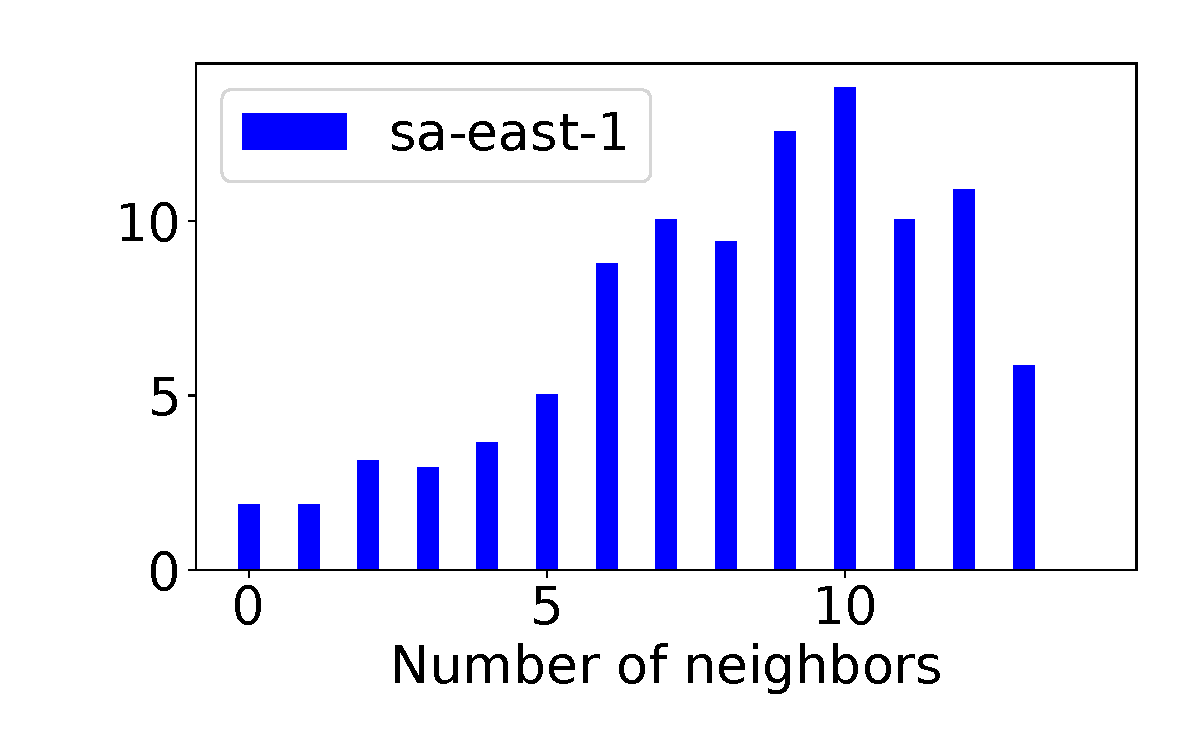
\includegraphics[width=.99\linewidth]{fig/colocation-sa-east-1.pdf}
  %   \caption{1b}
  %   \label{fig:sfig2}
  \end{subfigure}
  \begin{subfigure}{.33\textwidth}
    \centering
    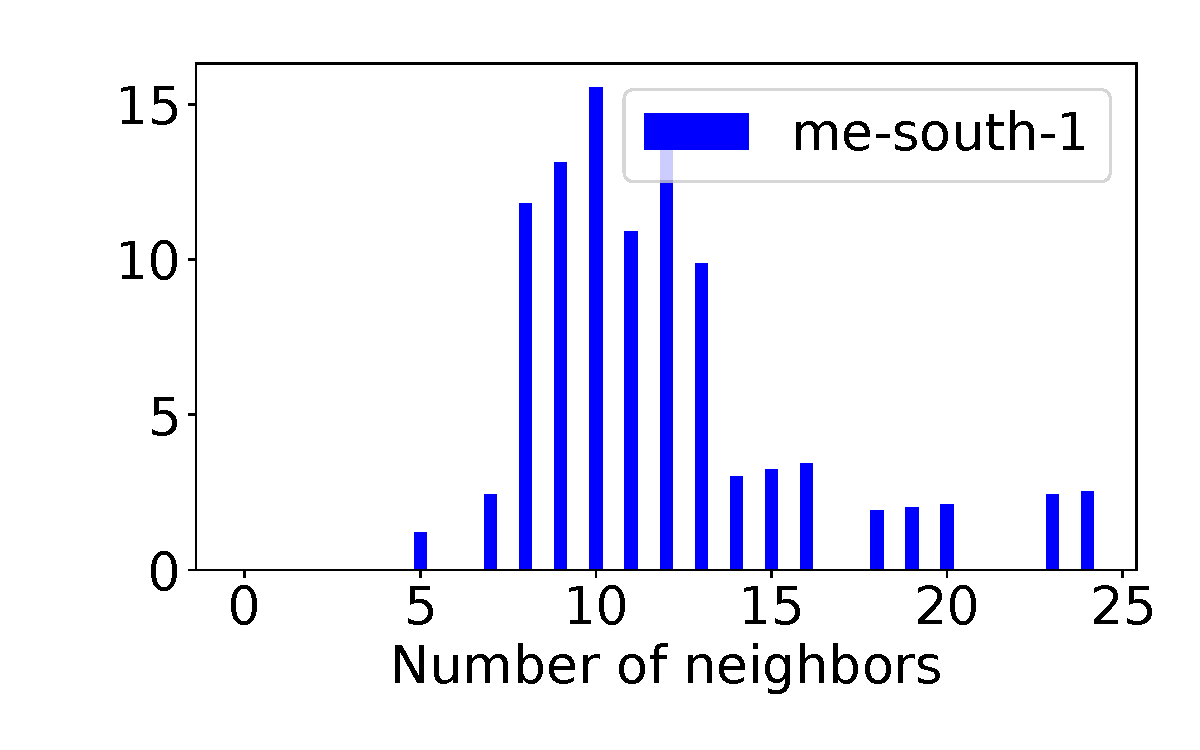
\includegraphics[width=.99\linewidth]{fig/colocation-me-south-1.pdf}
  %   \caption{1b}
  %   \label{fig:sfig2}
  \end{subfigure}
  \caption{We present co-residence results from a 1000-lambda run in different AWS regions. Each bar shows the fraction 
  of those 1000 lambdas (in \%) that discovered a certain number of neighbors. The total amount and density of co-residence 
  vary widely across regions, perhaps based on the size of those regions and the lambda activity within them. }
  \label{fig:awsregions}
  \end{figure*}

To demonstrate the correctness of our technique using this insight, we run an
experiment with 1000 1.5GB cold-started lambdas (ID'ed 1 to 1000) in one of
densest AWS regions (AWS MiddleEast), which resulted in many co-resident groups.
We repeat the experiment within a few seconds, thereby ensuring that all 1000
lambdas are warm-started on the second trial (i.e., they use the same set of
containers from the previous experiment).  For each co-resident group of lambdas
in the latter experiment, we observed that their predecessor lambdas (that used
the same set of containers) in the former experiment formed a co-resident group
as well.  That is, while the lambdas to the underlying container mapping is
different across both experiments, the results of the experiments agree
perfectly on the continer colocation. Figure~\ref{fig:correlation} shows that
both experiments saw the same number of co-residing groups of different sizes.
This proves the correctness of the results of our mechansim.

\subsubsection{Scalability}
One of the key properties of this technique is its execution speed. Since
communicating each binary bit of the ID takes one second, we are able to scale
the technique logarithmically with the number of lambdas involved.
Figure~\ref{fig:runtimes} shows this result with experiments involving
different number of lambdas. For example, in an experiment with 1000 lambdas,
each lambda can find its neighbors within a minute of its invocation, leaving
ample time for the attacker to then establish the covert channel and use it to 
send information. The logarithmic scale of our method also indicates that the 
cost per lambda scales logarithmically, making neighbor detection cost-effective.
\todo{note here about sublinear time?}
% mention cost of one run?




% Figures from the next section
% Moved here for formatting

\begin{figure}[!t]
  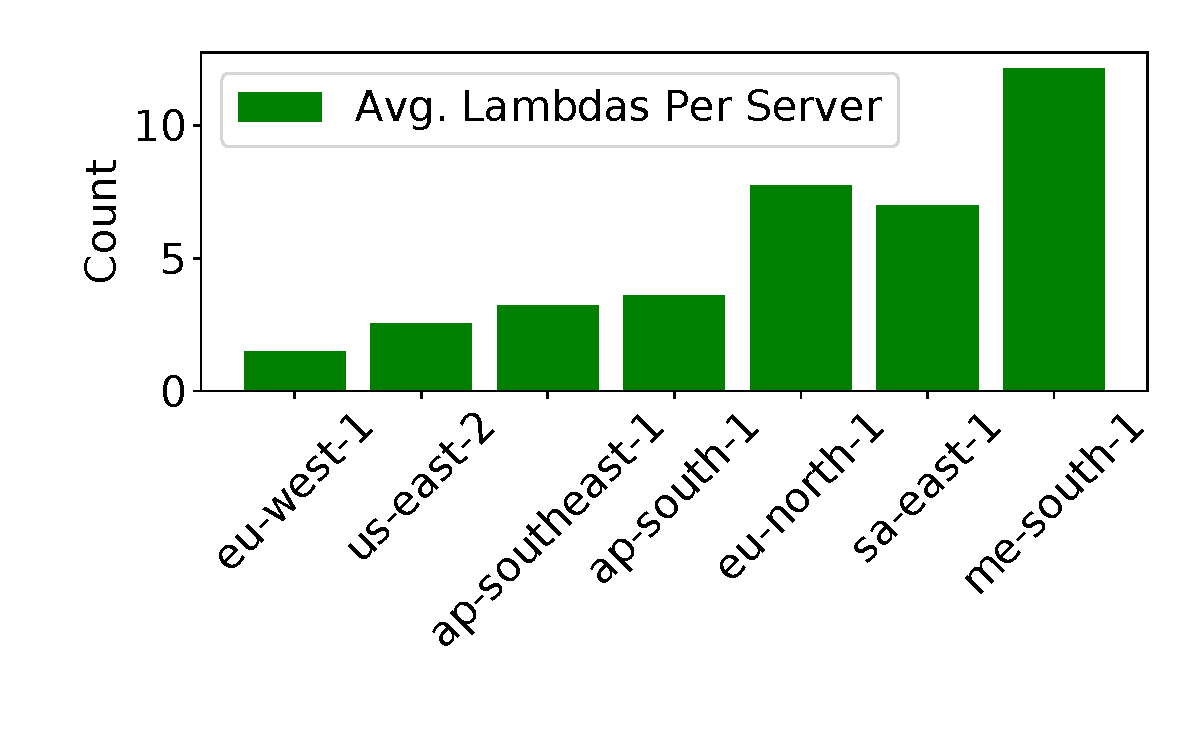
\includegraphics[width=.99\linewidth]{fig/density.pdf}
  \caption{This figure shows the average number of lambdas per server i.e., the co-residence 
  density seen in various AWS regions for the runs shown in Figure~\ref{fig:awsregions}. 
  The ample co-residence across regions demonstrates the practicality of establishing 
  covert channels with lambdas in these regions.
\label{fig:density}}
\end{figure}

%\paragraph{Generality}
%\todo{We only implemented it on AWS. This requires us to implement it on 
%Azure and GCP, and report some results. \textbf{Needs considerable effort}}
